\documentclass[../../../../main.tex]{subfiles}
\begin{document}

\begin{flushright}
\footnotesize\textit{【自動文字起こし・要確認】}
\end{flushright}

[解]右のような座標をおく。対称性から、
楕円の中心 $D(0,a)$ とすると、$b>0$ として、
楕円の方程式は
\[ \frac{x^2}{b^2} + \frac{(y-a)^2}{a^2} = 1 \]
とかける。($\because$ BCと接し、軸がBCと平行) ここで、$X=\frac{x}{b}$、$Y=\frac{y}{a}$ なる変換を行うと、
楕円は
\[ P : X^2 + (Y-1)^2 = 1 \]
へ、直線AB: $x+y=1$ は、
\[ l : bX + aY = 1 \]
へ、各々うつる。以下、ABと楕円が接する条件をかんがえる。(対称性から、この時ACと楕円が接する条件も同じ)。
$l$ と $(0,1)$ のキョリが $1$ なら良いので、
\[ \frac{|a-1|}{\sqrt{a^2+b^2}} = 1 \]
両辺 $0$ 以上から2乗して、
\[ b^2 = 1 - 2a \cdots \text{①} \]

ここで、$a$ は $0 < a = \frac{1-b^2}{2} < 1 \iff 0 < 1-b^2 < 2 \implies b^2 < 1$ から
$0 < b < 1 \cdots \text{②}$ をみたす。

楕円の面積 $S$ は、
\[ S = \pi a b = \pi b \frac{1-b^2}{2} \quad (\because \text{①}) \]
である。$f(b) = b(1-b^2)$ とすると、$f'(b) = 1 - 3b^2$ から、下表をうる。

\begin{center}
\begin{tabular}{|c|c|c|c|c|c|}
\hline
$b$ & $0$ & $\cdots$ & $\frac{1}{\sqrt{3}}$ & $\cdots$ & $1$ \\
\hline
$f'$ & & $+$ & $0$ & $-$ & \\
\hline
$f$ & & $\nearrow$ & & $\searrow$ & \\
\hline
\end{tabular}
\end{center}

したがって、$S$ は $b = \frac{1}{\sqrt{3}}$ で最大値、$\frac{\pi}{2} \cdot \frac{1}{\sqrt{3}} \cdot \frac{2}{3} = \frac{\sqrt{3}}{9}\pi$ をとる。
\begin{flushright}
(終)
\end{flushright}

\begin{center}
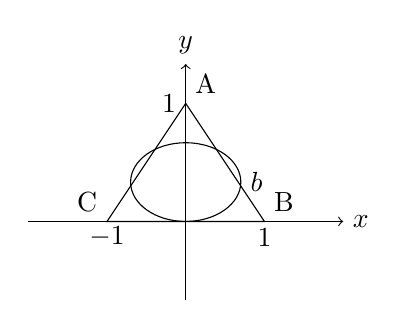
\begin{tikzpicture}
\draw[->] (-2,0) -- (2,0) node[right] {$x$};
\draw[->] (0,-1) -- (0,2) node[above] {$y$};
\draw (-1,0) -- (1,0) -- (0,1.5) -- cycle;
\node at (-1,-0.2) {$-1$};
\node at (1,-0.2) {$1$};
\node at (0,1.5) [left] {$1$};
\node at (-1,0) [above left] {C};
\node at (1,0) [above right] {B};
\node at (0,1.5) [above right] {A};
\draw (0,0.5) ellipse (0.7 and 0.5);
\node at (0.7,0.5) [right] {$b$};
\end{tikzpicture}
\end{center}

\end{document}
